%! TEX root = 'main.tex'
\section{Background}
\label{sec:background}


The term Industrial Control System (ICS) describes different control systems and associated instrumentation, including the devices, systems, networks, and controls used to operate and automate industrial processes. Supervisory Control and Data Acquisition (SCADA) systems and Distributed Control Systems (DCS) are the most common ICS. The ICS connects sensors and actuators that interact with the physical systems (e.g., power grid) with the cyber components such as networks and servers. Local operations are often controlled by so-called Field Devices that receive supervisory commands from remote stations. Whether it has remote communication components, the controller field devices are categorized as Programmable Logic Controller (PLC) and Remote Terminal Unit (RTU). They are used in both DCS and SCADA systems as a control component of an overall system. 

\textbf{\textit{PLC}}. PLCs consist of a processor, I/O modules, a power supply, and other specialized addon modules. The I/O modules of PLCs interact with the physical world, gathering digital inputs from sensors, switch, or a thermometer. The processor servers the PLC's brain executes pre-programmed ladder logic based on the inputs and gives operation signals through the output module. That said, it is not easy to tell the difference between a PLC and an embedded system. Usually, they both use a microcontroller as the processor. PLCs are designed and rigorously tested to withstand operating in an industrial environment where they may be exposed to vibration and noise. 

With an embedded system solution, the choice of the microcontroller is various. Moreover, each system has its own specialized circuit board design around it. On the contrary, several major PLC vendors dominate the market so that only numerous models are widely used, and particular programming tool-chain such as ladder logic is used. Therefore, from the attacker's perspective, anyone who purchases the same-model PLC will have the exact hardware and software environment as the target system.

The PLC has a firmware acting as the real-time operating system. It also provides library routines to operate on various I/O devices such as I2C and SPI. These routines may reside at fixed addresses of the ROM. The firmware loads the control logic, such as a compile ladder logic binary at bootstrap or each update initiated from the remote operator.

The ladder logic programs are executed repeatedly in fixed intervals, called scan cycles. When the logic calls the firmware routines to toggle an output pin, it is carried out by setting/clearing a memory bit, which is the MMIO address corresponding to output pins, thus to the sockets of the I/O module. PLC usually has LEDs at the front panel to indicate the inputs and output pins' current status.


\textbf{\textit{JTAG}} is a common name of the industry-standard IEEE1149.1 for verifying designs and testing printed circuit boards after manufacture. It is named after the Joint Test Action Group.

JTAG is the common name of the IEEE1149.1 standard, which defines the Standard Test Access Port and Boundary-Scan Architecture for test access ports used for testing printed circuit boards using boundary scan. The JTAG interface uses very few pins (TDI, TDO, TMS, TCK, and TRST) to connect to an on-chip Test Access Port (TAP) that implements a stateful protocol, as shown in ~\autoref{fig:jtagsm}.  One or more devices can expose multiple TAPs in a daisy chain, also known as a scan chain. The host communicates with the TAPs by manipulating TMS and TDI in conjunction with TCK and reading results through TDO. 

\begin{figure}[ht]
	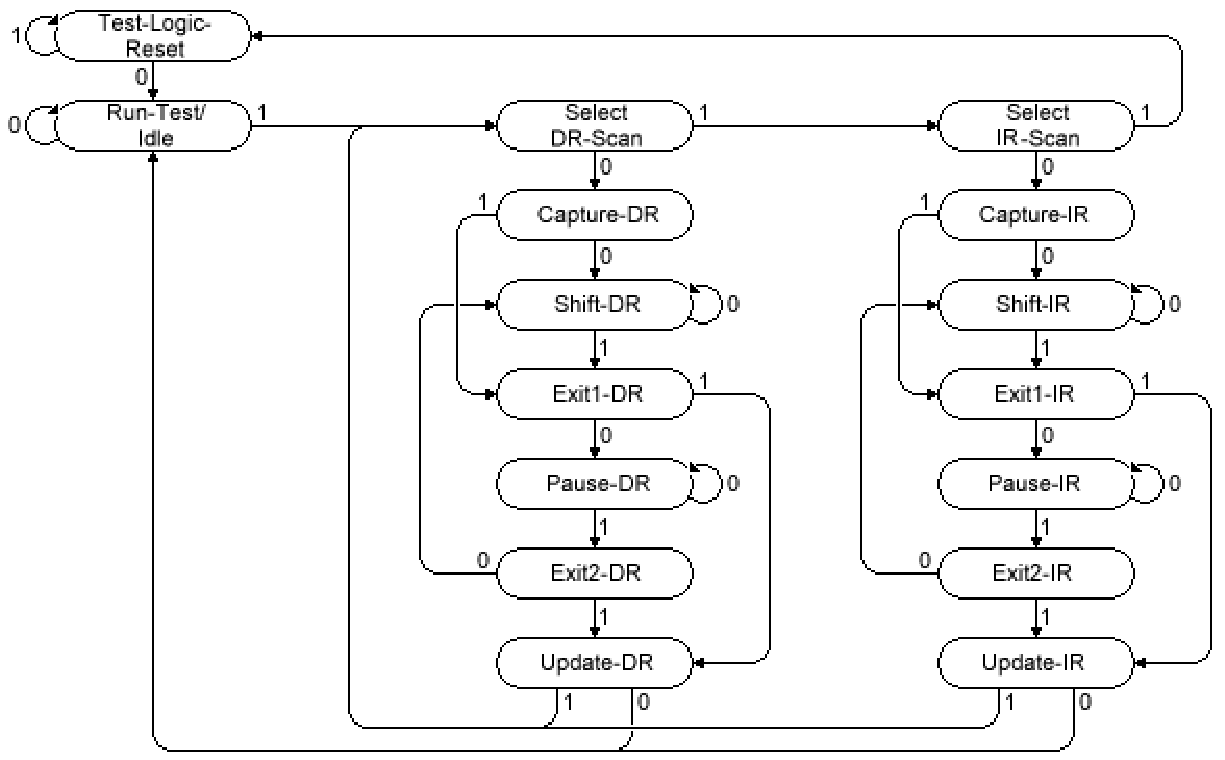
\includegraphics[width=0.47\textwidth]{figures/jtagsm}
	\centering
	\caption{JTAG TAP state machine.}
	\label{fig:jtagsm}
\end{figure}


The JTAG standard has four common registers: Instruction Register (IR) and Data Register (DR),  IDCODE, and BYPASS. The IDCODE register contains data that uses a standardized format that includes a manufacturer code. The BYPASS register is a single bit data register that allows this device to be bypassed (do nothing) while other devices in the scan chain are examined. The IR and DR register's size depends on the TAP implementation, and they are used to send in instruction and receive result data.

The TAP implementation defines various instructions, as are data registers associated. For example, the host sends in the IDCODE instruction through IR and subsequently gets the value of the same-name 32-bit register (IDCODE) from TDO.

The target device we have been worked on uses an ARM core, and the TAP controller is also implemented using CoreSight technologies from ARM. It is called Debug Access Port (DAP) instead. One of the differences is that, traditionally, accessing system memory would be achieved by halting the processor and then downloading instructions. On the other side, the CoreSight DAP controller implements a bridge between the external and various on-chip protocols so that one can access memory at run time. 

\begin{figure}[ht]
	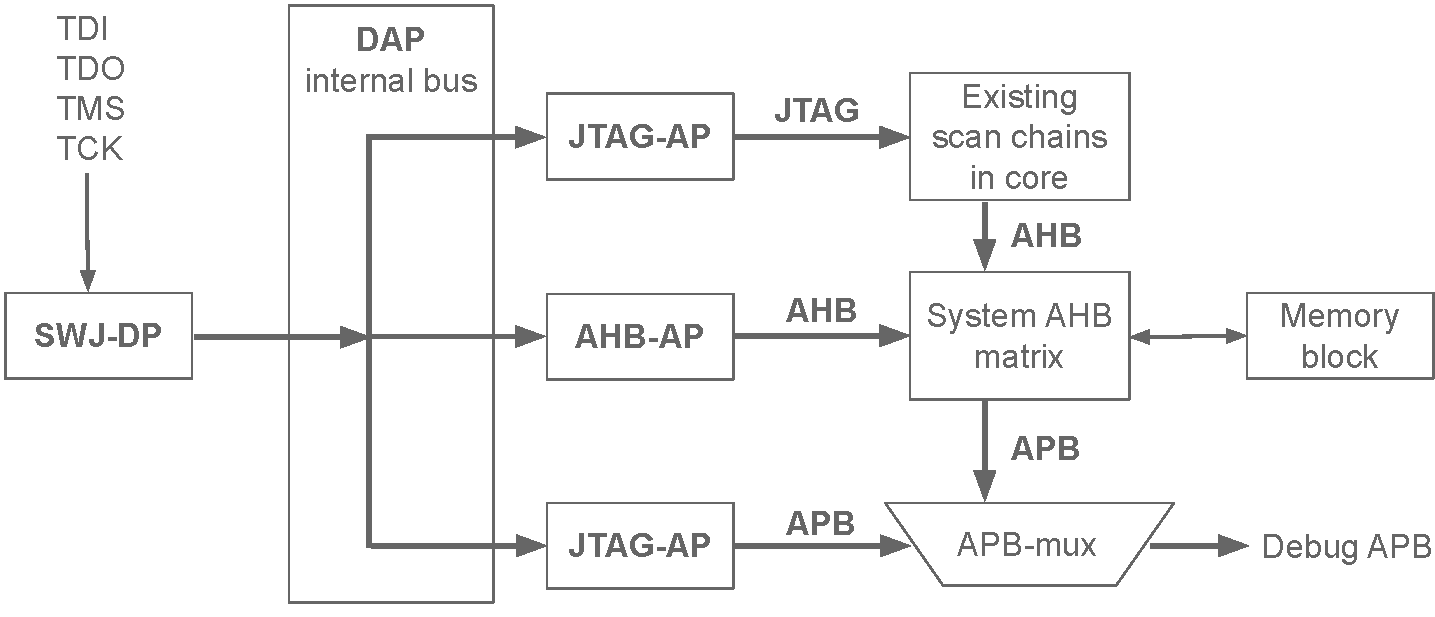
\includegraphics[width=0.47\textwidth]{figures/dap}
	\centering
	\caption{The debug port receives host signals and maintains the JTAG state machine. Through IR and DR, instruction and data are sent in, and specific registers are utilized to access on-device resources. SRAM and MMIO memory on the ARM microcontroller can be accessed through the AHB bus at runtime without halting the processor.}
	\label{fig:dap}
\end{figure}

As shown in~\autoref{fig:dap}, each DAP contains Debug Ports (DPs) and Access Ports (APs). The DP  accesses the DAP from an external debugger and controls the APs to respond to external commands to access on-chip system resources. In this case, the DP port used is Serial Wire JTAG Debug Port (SWJ-DP) since the interface supports both JTAG and Serial Wire (DW) protocols.
For system accesses, the access ports are AHP-AP, ABP-AP, and JTAG-AP. The AHB-AP provides an AHB-Lite master for access to a system AHB bus, which we primarily use to access the RAM or MMIO of the PLC. 


Because of this comprehensive debug ability that the ARM CoreSight DAP controller provides, our hardware implant can fully control it by connecting to the JTAG pins.


